

\section{Overflow mode: RUN281}
%%%%%%%%%%%%%%%%%%%%%%%%%%%%%%%%%%%%%%%%%%%%%%%%%%%%%%%%%%%%%%%%%%%%%%%%%%%%%%
\subsection{Time distribution and Occupancy}\label{over}
The first distributions to look at are the time distribution of hits in a specific channel and the occupancy distribution (total number of hits in function of the channel number).
The timing distributions of hits in different channels are shown in Fig.\ref{fig:1}.
These pictures show the timing distribution of hits in channel 0 of the first FPGA and in channel 2 of the second FPGA.
The left one is uniform, however the right one looks non trivial.

\begin{figure}[H]
  \hspace{-0.5in}
  \begin{tikzpicture}
    \node[anchor=south west,inner sep=0] at (0,0.) {
      % \node[shift={(0 cm,0.cm)},inner sep=0,rotate={90}] at (0,0) {}
      % \makebox[\textwidth][c] {
      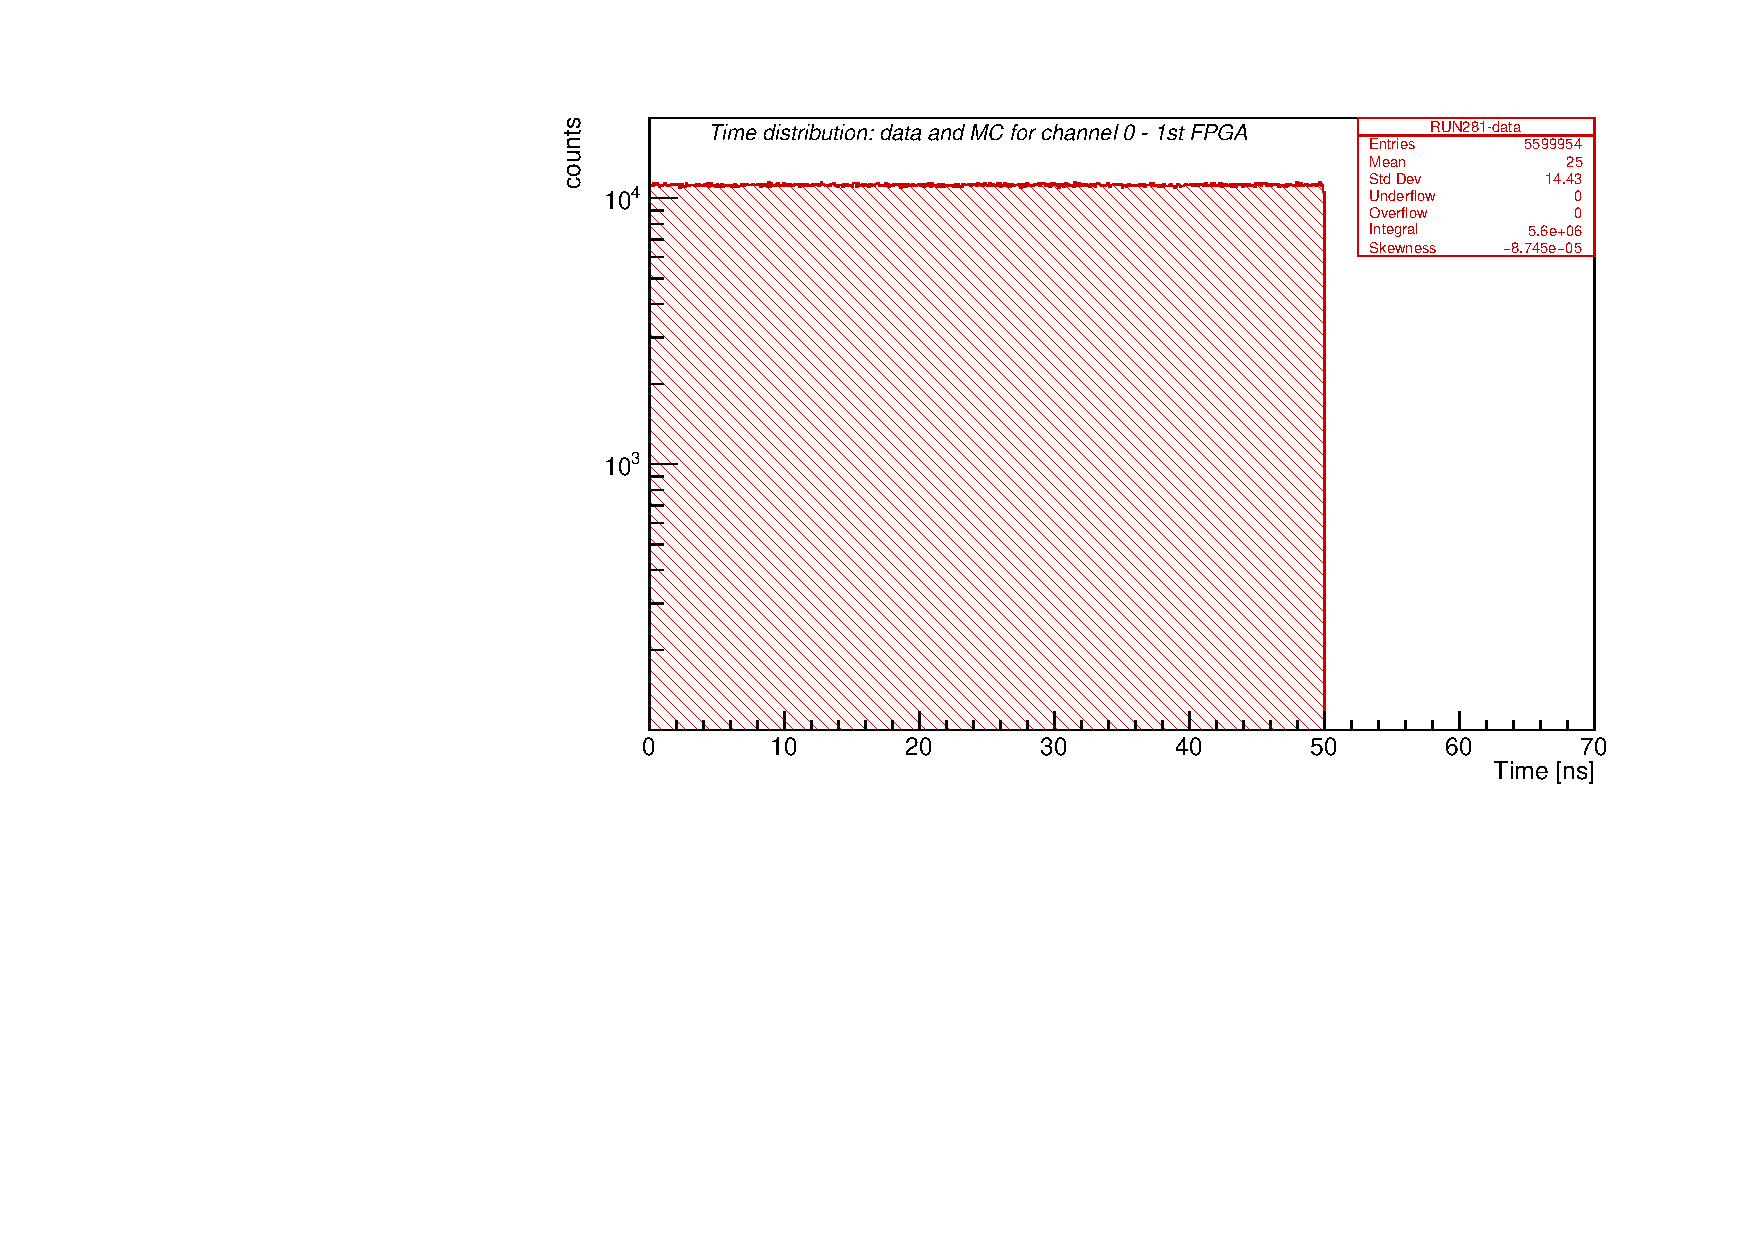
\includegraphics[width=0.5\textwidth]{figures/pdf/figure_00007_timedistr_roc_simulation_ch0_281}
      % }
    };
    \node[anchor=south west,inner sep=0] at (10,0.) {
      % \node[shift={(0 cm,0.cm)},inner sep=0,rotate={90}] at (0,0) {}
      % \makebox[\textwidth][c] {
      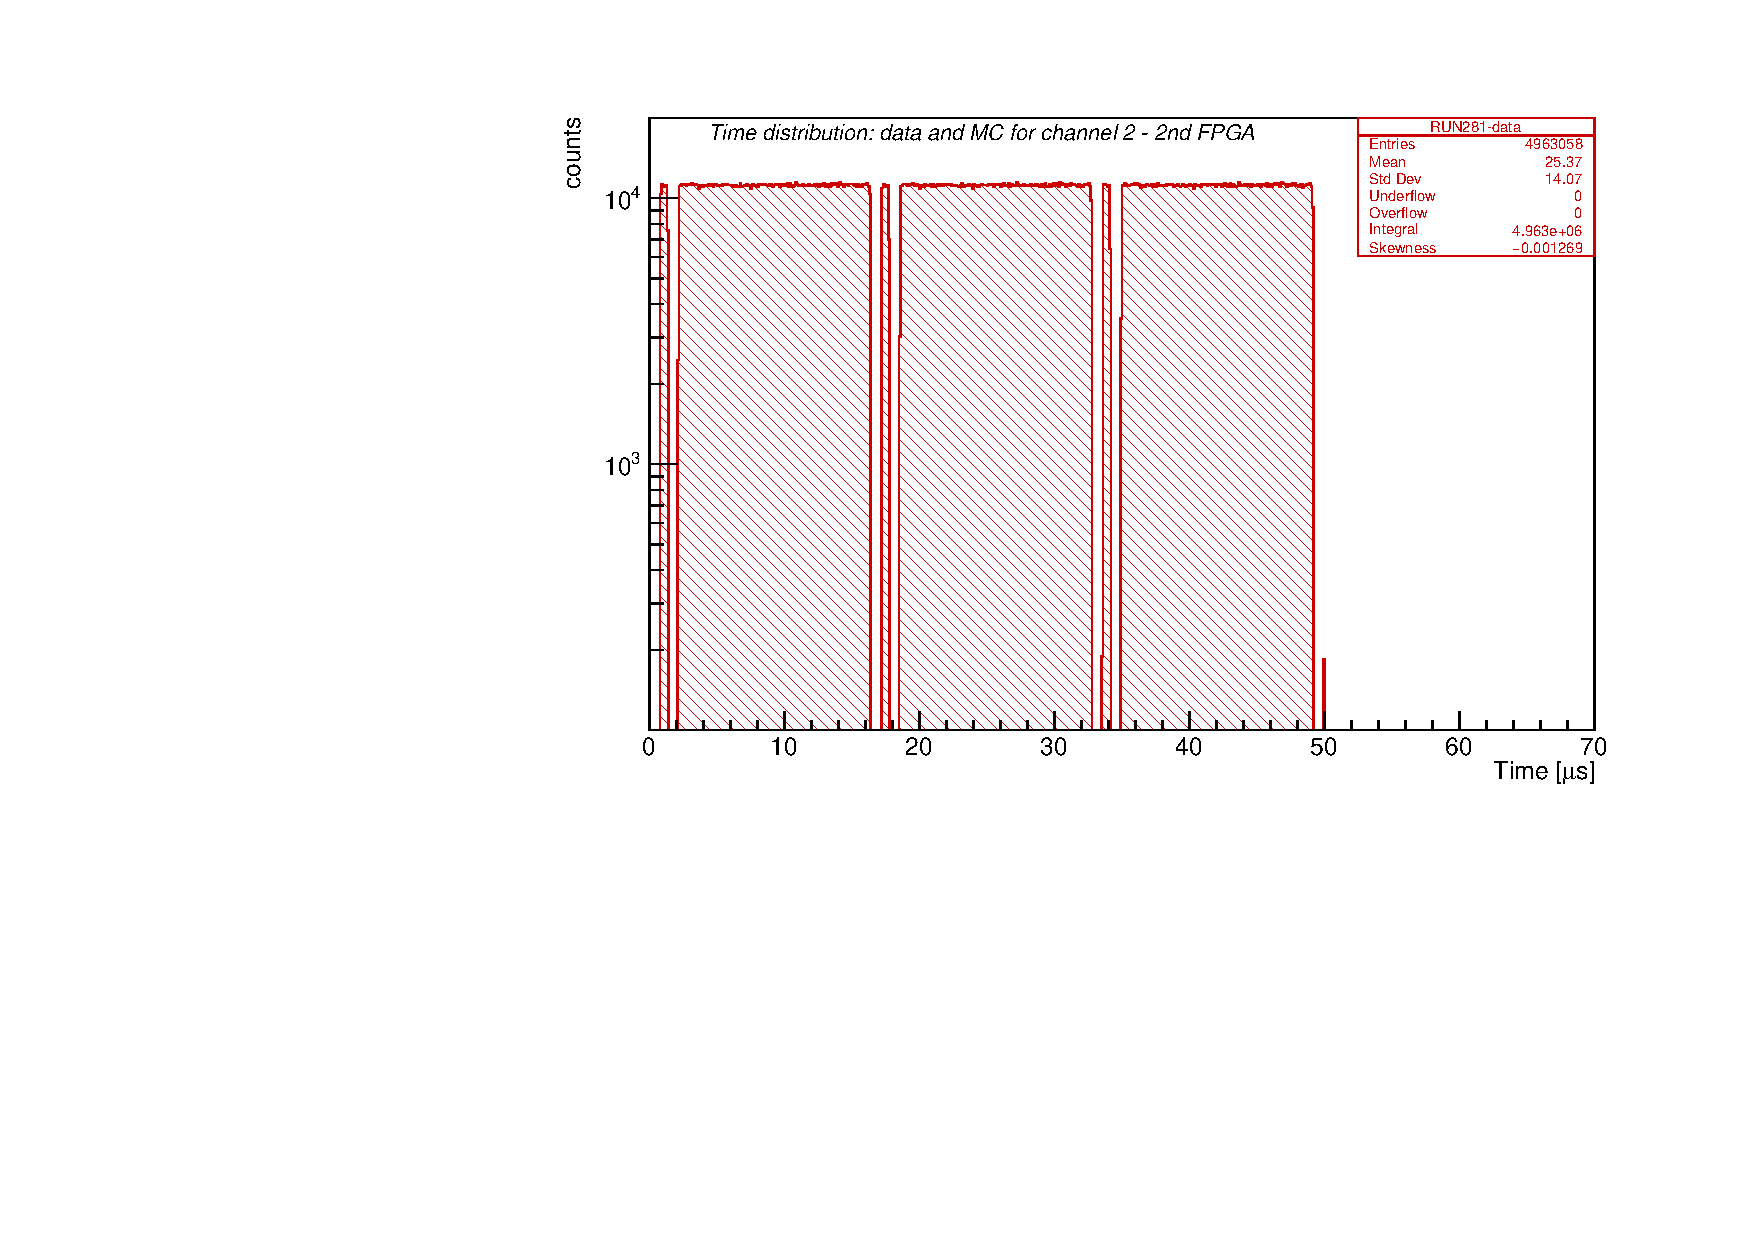
\includegraphics[width=0.5\textwidth]{figures/pdf/figure_00003_timedistr_roc_simulation_ch2_281}
      % }
    };
  \end{tikzpicture}
  \caption{
    \label{fig:1}
    left: channel 0 (first FPGA) time distribution of hits, right: channel 2 (second FPGA) time distribution of hits.
  }
\end{figure}

The distributions in Fig.\ref{fig:1} are easier to understand by looking at the occupancy plot in Fig.\ref{fig:2} (left one). Channel ordering in this plot corresponds to the readout order.
This revealed a non uniform distribution. We compared with the Monte Carlo occupancy.
\begin{figure}[H]
  \hspace{-0.5in}
  \begin{tikzpicture}
    \node[anchor=south west,inner sep=0] at (0,0.) {
      % \node[shift={(0 cm,0.cm)},inner sep=0,rotate={90}] at (0,0) {}
      % \makebox[\textwidth][c] {
      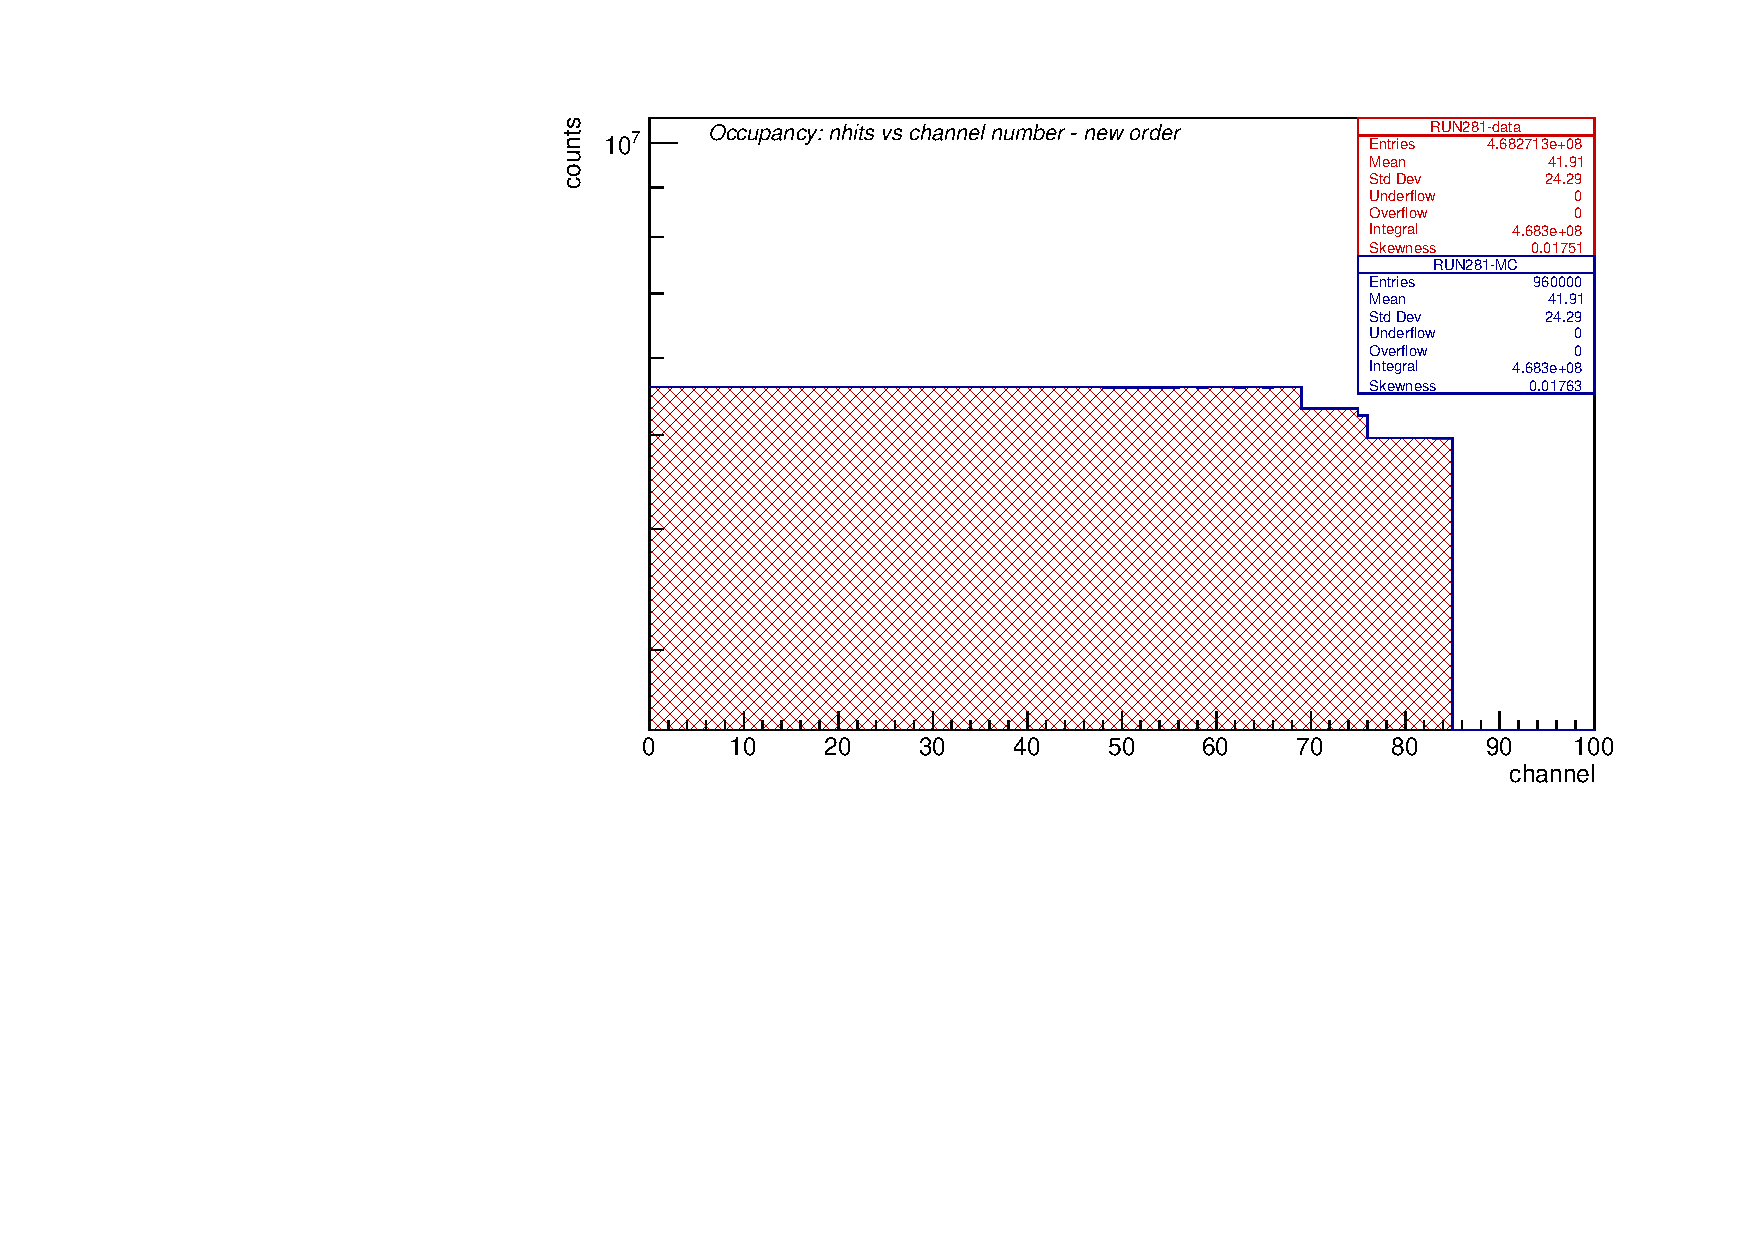
\includegraphics[width=0.5\textwidth]{figures/pdf/figure_00004_nhitsvschannel_roc_simulation_281}
      % }
    };
    \node[anchor=south west,inner sep=0] at (10,0.) {
      % \node[shift={(0 cm,0.cm)},inner sep=0,rotate={90}] at (0,0) {}
      % \makebox[\textwidth][c] {
      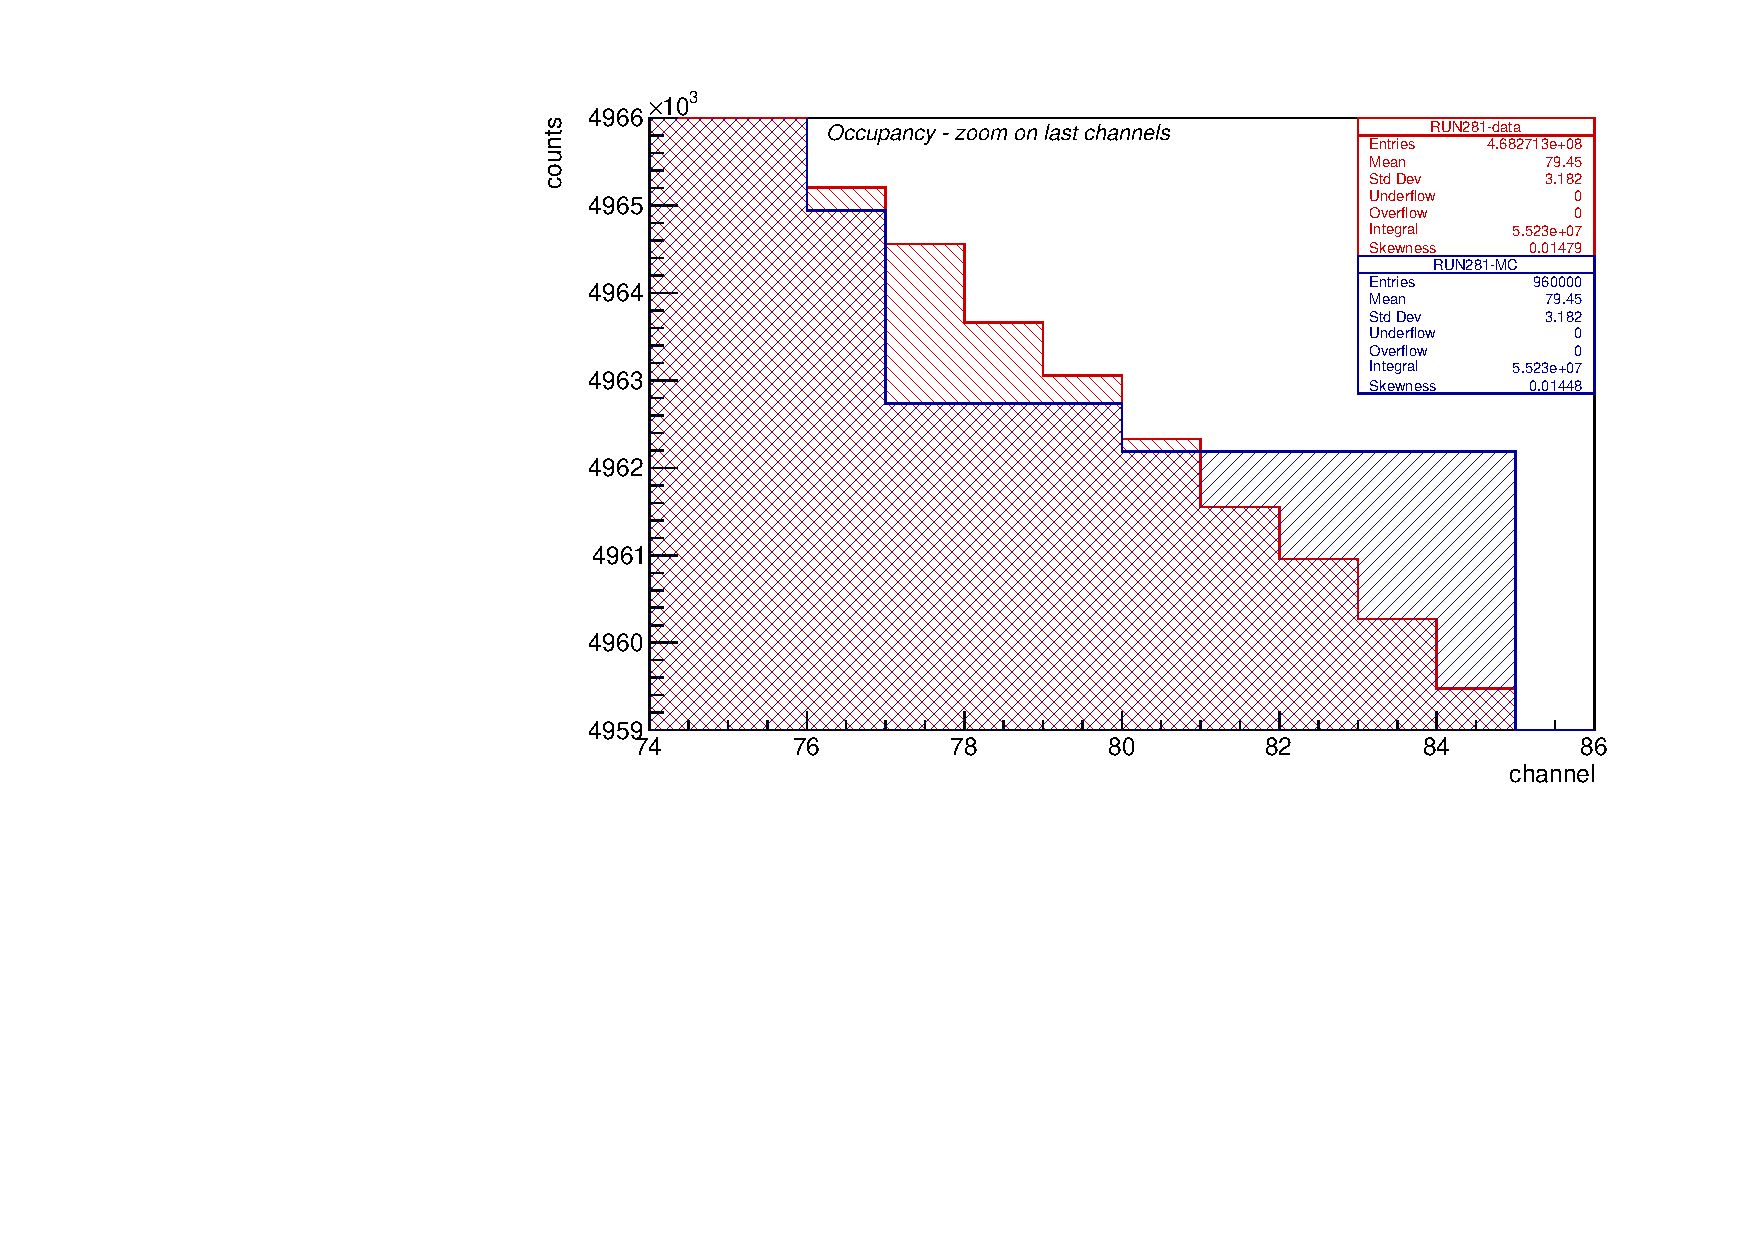
\includegraphics[width=0.5\textwidth]{figures/pdf/figure_00014_nhitsvschannel_roc_simulation_281}
      % }
    };
  \end{tikzpicture}
  \caption{
    \label{fig:2}
    left: number of hits versus channel. The ordering of channels adheres to the sequence prescribed by the Monte Carlo simulation, right: zoom on last channels. The two histrograms differ from each other of a value <10$^{-3}$.
  }
\end{figure}
To understand occupancy plot, the number of hits per channel has a key role. In Fig.\ref{fig:66} the number of hits (data) in channel 0 is shown. In this configuration there could be 3 or 4 hits per channel, as for the other ones.
\begin{figure}[H]
\centering
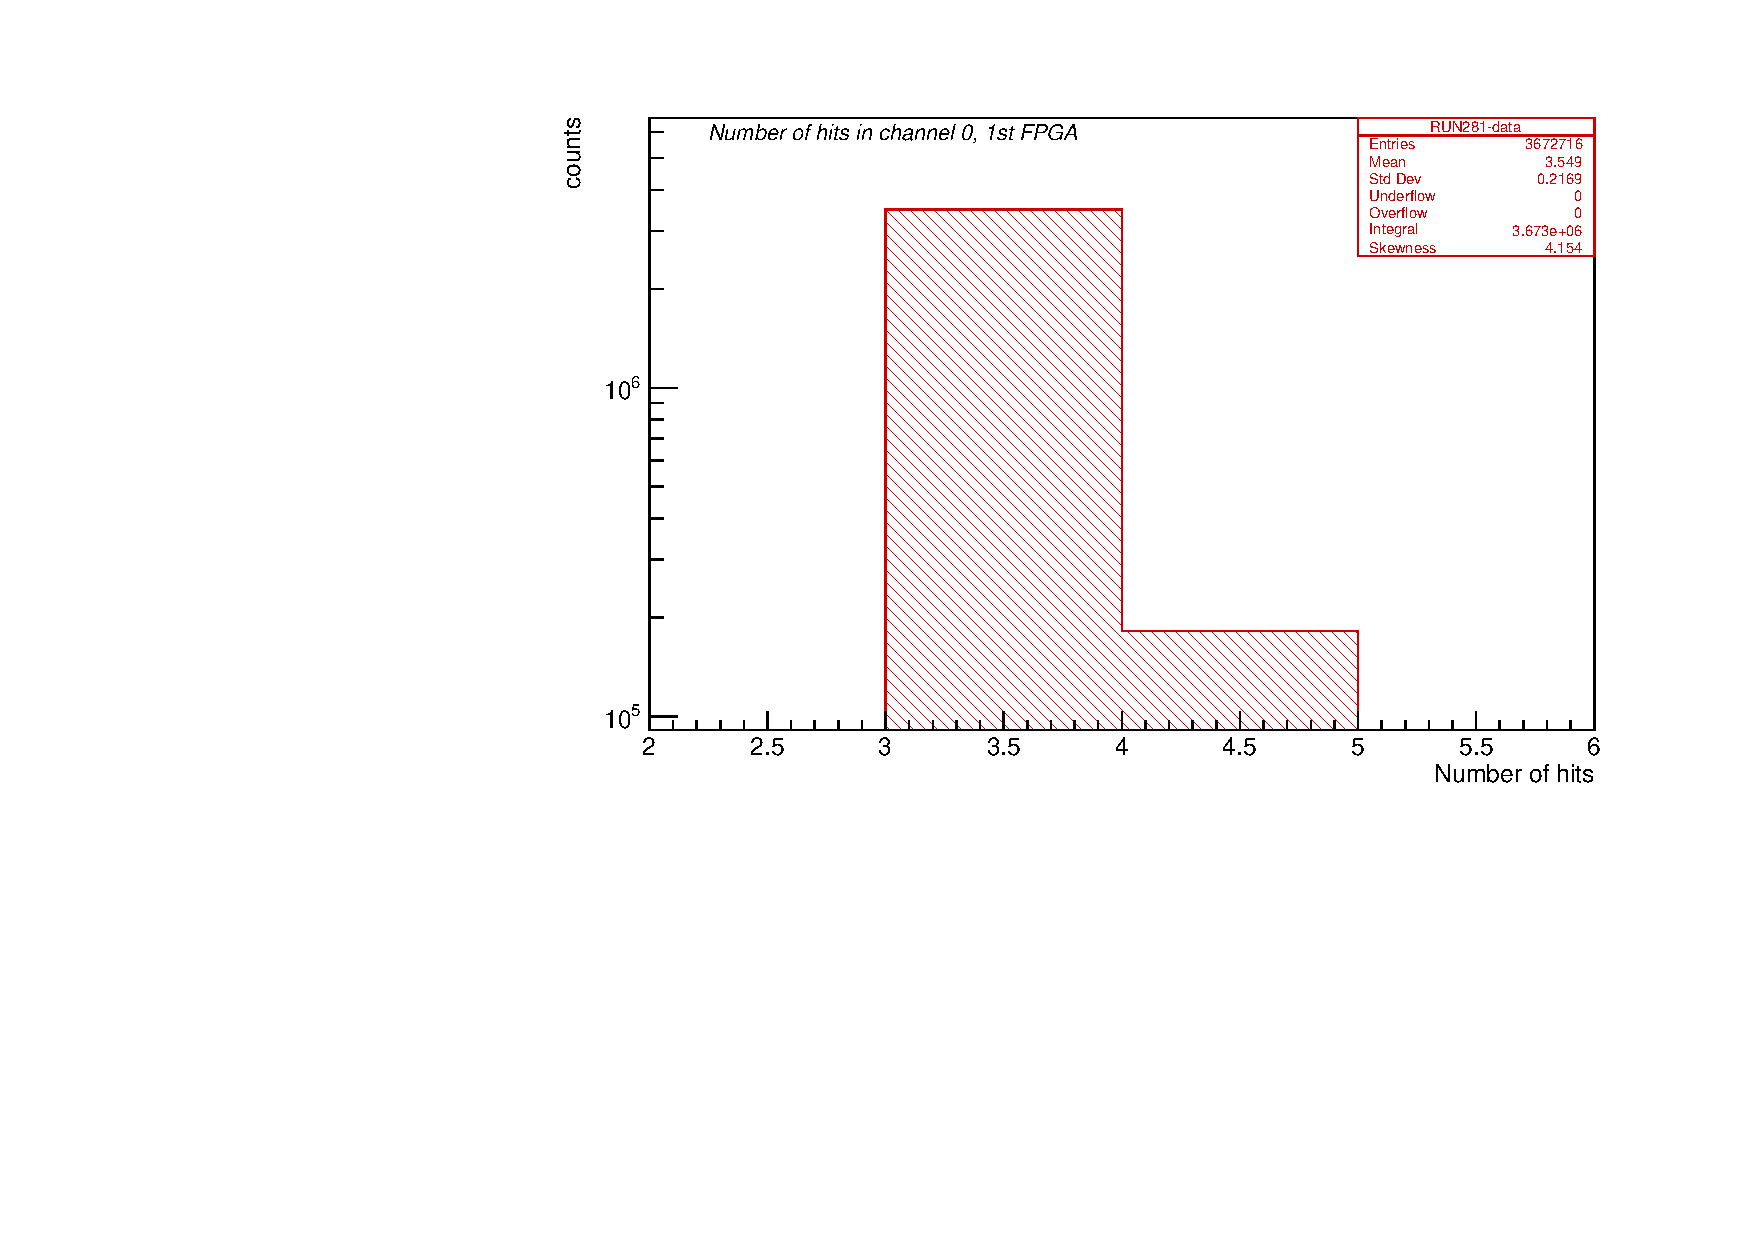
\includegraphics[width =0.8\textwidth]{figures/pdf/figure_00066_nhits_ch00_run281.pdf}
\caption{Number of hits per channel. It is shown that in this configuration there could be 3 or 4 hits in channel 0, as in other channels.}
\label{fig:66}
\end{figure}

In the left picture of Fig.\ref{fig:2}, the first 68 channels are the ones with 4 hits in the first FPGA and three in the second FPGA, achieving in total 255 hits. The second plateau extending from 68 to 75 is composed by the channels with 3 hits in the first FPGA and 4 hits in the second one. There is a big step at the end of this plateau, because if we count the number of hits in the first FPGA we get 144, so in the second FPGA we have 111 hits in total, due to the fact that the maximum number of hits in total is 255. 111 is not divisible by 4, so the first 27 channels in the second FPGA will have 4 hits and the last one will have 3 hits. Last plateau consists of 3 hits from the first FPGA and 3 hits from the second FPGA. A zoom on last channels is shown on the right picture of Fig.\ref{fig:2}. The two histograms differ from each other of a value $<10^{-3}$: this is a good agreement. The differences are due to the fact that each FPGA has its own pulse generator and pulse sequences from different generators are offset with respect to each other by a random number and also timing of generator pulses are uncorrelated with the beginning of the time window. Coming back to Fig.\ref{fig:1}, some channels are always readout and some others no, as we explained in the introduction the ROC hit buffer gets filled up and only the first 255 hits are read out. This results in a uniform time distribution for the first channels readout and in a non uniform time distribution for the last readout channels, depending on $T_{gen}$ and $T_{EW}$. The deeps in channel 2 are defined by the differences between the two pulsers. 

\subsection{Number of hits}
 Fig. \ref{fig:3} shows that we are reading out 255 hits as expected.
\begin{figure}[!h]
\centering
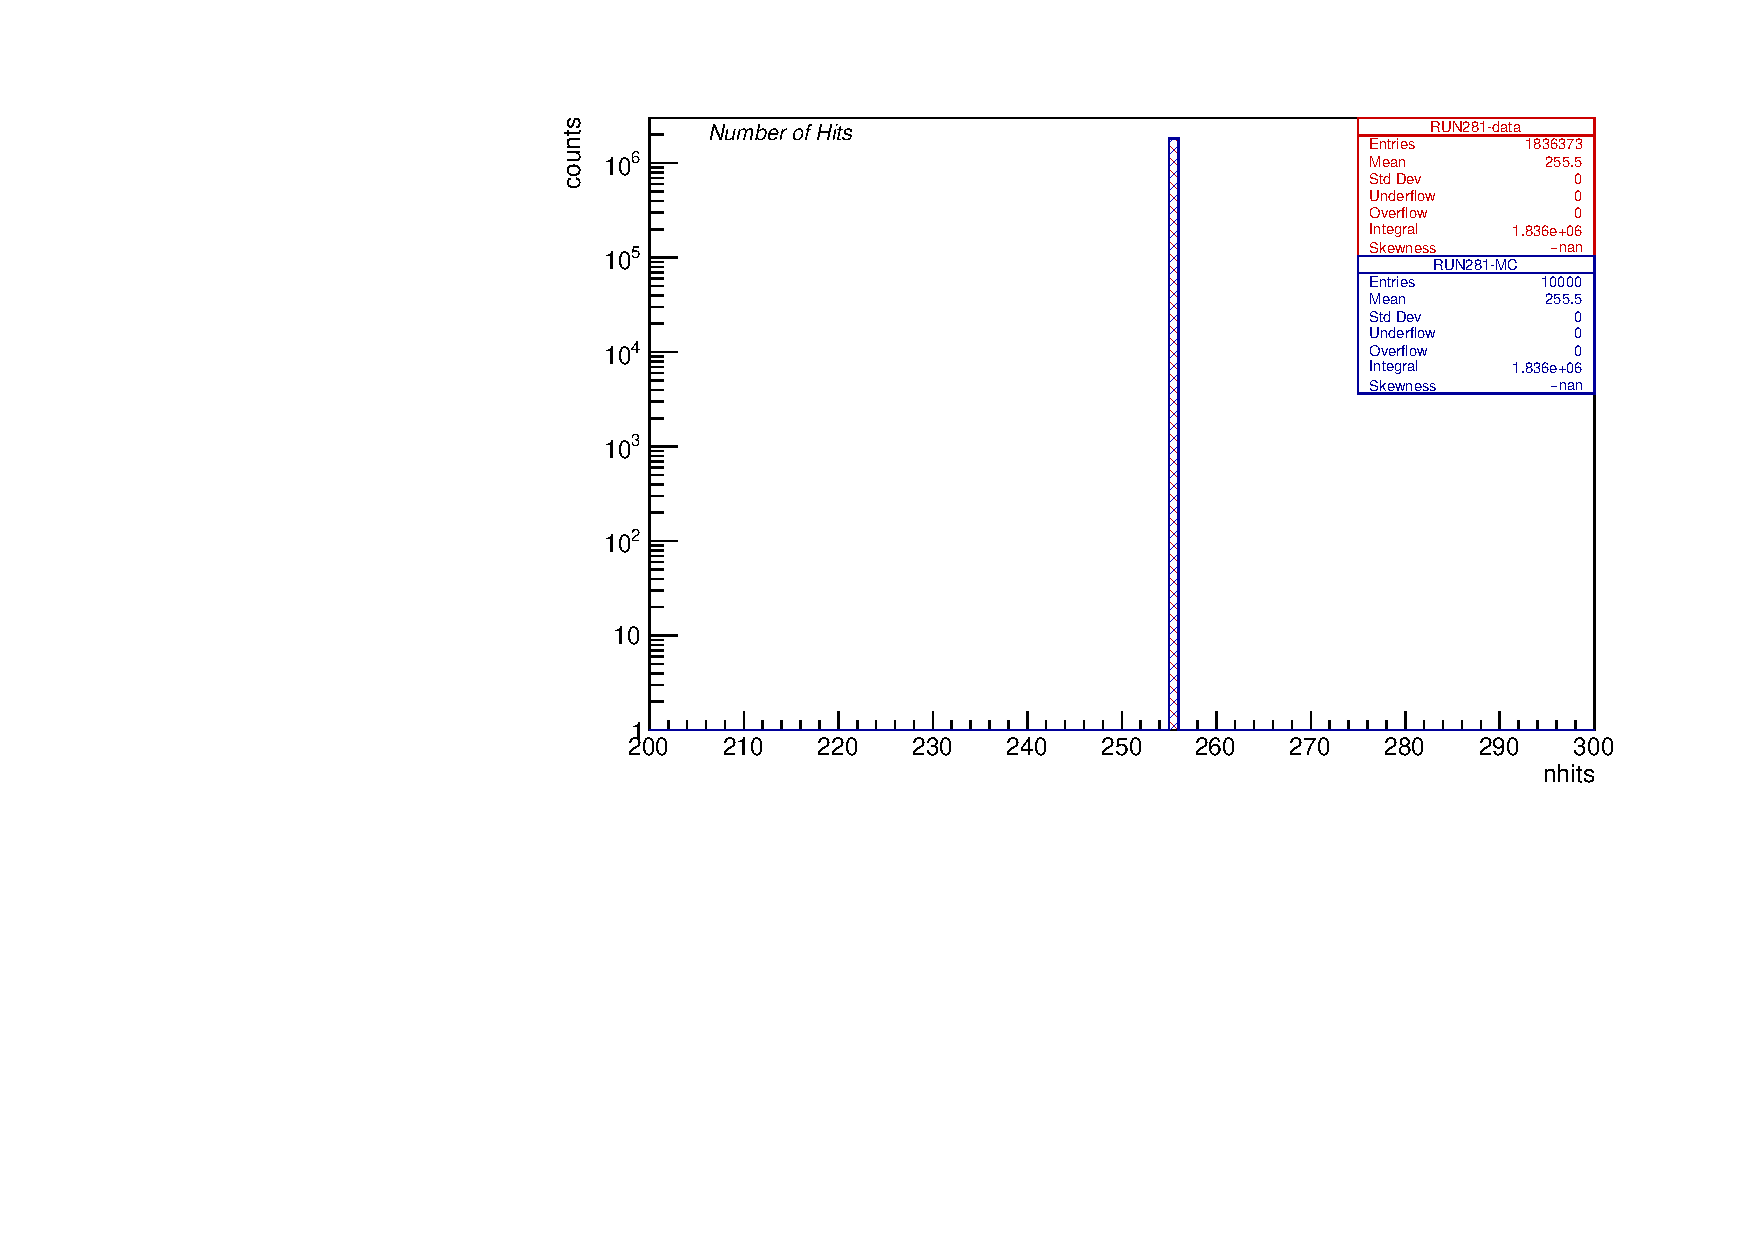
\includegraphics[width =0.8\textwidth]{figures/pdf/figure_00008_nhits_281}
\caption{Total number of hits distribution.}
\label{fig:3}
\end{figure}


%%% Local Variables:
%%% mode: latex
%%% TeX-master: t
%%% End:
